\documentclass[twoside]{book}

% Packages required by doxygen
\usepackage{fixltx2e}
\usepackage{calc}
\usepackage{doxygen}
\usepackage[export]{adjustbox} % also loads graphicx
\usepackage{graphicx}
\usepackage[utf8]{inputenc}
\usepackage{makeidx}
\usepackage{multicol}
\usepackage{multirow}
\PassOptionsToPackage{warn}{textcomp}
\usepackage{textcomp}
\usepackage[nointegrals]{wasysym}
\usepackage[table]{xcolor}

% Font selection
\usepackage[T1]{fontenc}
\usepackage[scaled=.90]{helvet}
\usepackage{courier}
\usepackage{amssymb}
\usepackage{sectsty}
\renewcommand{\familydefault}{\sfdefault}
\allsectionsfont{%
  \fontseries{bc}\selectfont%
  \color{darkgray}%
}
\renewcommand{\DoxyLabelFont}{%
  \fontseries{bc}\selectfont%
  \color{darkgray}%
}
\newcommand{\+}{\discretionary{\mbox{\scriptsize$\hookleftarrow$}}{}{}}

% Page & text layout
\usepackage{geometry}
\geometry{%
  a4paper,%
  top=2.5cm,%
  bottom=2.5cm,%
  left=2.5cm,%
  right=2.5cm%
}
\tolerance=750
\hfuzz=15pt
\hbadness=750
\setlength{\emergencystretch}{15pt}
\setlength{\parindent}{0cm}
\setlength{\parskip}{3ex plus 2ex minus 2ex}
\makeatletter
\renewcommand{\paragraph}{%
  \@startsection{paragraph}{4}{0ex}{-1.0ex}{1.0ex}{%
    \normalfont\normalsize\bfseries\SS@parafont%
  }%
}
\renewcommand{\subparagraph}{%
  \@startsection{subparagraph}{5}{0ex}{-1.0ex}{1.0ex}{%
    \normalfont\normalsize\bfseries\SS@subparafont%
  }%
}
\makeatother

% Headers & footers
\usepackage{fancyhdr}
\pagestyle{fancyplain}
\fancyhead[LE]{\fancyplain{}{\bfseries\thepage}}
\fancyhead[CE]{\fancyplain{}{}}
\fancyhead[RE]{\fancyplain{}{\bfseries\leftmark}}
\fancyhead[LO]{\fancyplain{}{\bfseries\rightmark}}
\fancyhead[CO]{\fancyplain{}{}}
\fancyhead[RO]{\fancyplain{}{\bfseries\thepage}}
\fancyfoot[LE]{\fancyplain{}{}}
\fancyfoot[CE]{\fancyplain{}{}}
\fancyfoot[RE]{\fancyplain{}{\bfseries\scriptsize Generated by Doxygen }}
\fancyfoot[LO]{\fancyplain{}{\bfseries\scriptsize Generated by Doxygen }}
\fancyfoot[CO]{\fancyplain{}{}}
\fancyfoot[RO]{\fancyplain{}{}}
\renewcommand{\footrulewidth}{0.4pt}
\renewcommand{\chaptermark}[1]{%
  \markboth{#1}{}%
}
\renewcommand{\sectionmark}[1]{%
  \markright{\thesection\ #1}%
}

% Indices & bibliography
\usepackage{natbib}
\usepackage[titles]{tocloft}
\setcounter{tocdepth}{3}
\setcounter{secnumdepth}{5}
\makeindex

% Hyperlinks (required, but should be loaded last)
\usepackage{ifpdf}
\ifpdf
  \usepackage[pdftex,pagebackref=true]{hyperref}
\else
  \usepackage[ps2pdf,pagebackref=true]{hyperref}
\fi
\hypersetup{%
  colorlinks=true,%
  linkcolor=blue,%
  citecolor=blue,%
  unicode%
}

% Custom commands
\newcommand{\clearemptydoublepage}{%
  \newpage{\pagestyle{empty}\cleardoublepage}%
}

\usepackage{caption}
\captionsetup{labelsep=space,justification=centering,font={bf},singlelinecheck=off,skip=4pt,position=top}

%===== C O N T E N T S =====

\begin{document}

% Titlepage & ToC
\hypersetup{pageanchor=false,
             bookmarksnumbered=true,
             pdfencoding=unicode
            }
\pagenumbering{roman}
\begin{titlepage}
\vspace*{7cm}
\begin{center}%
{\Large Trick Variable Server Connection -\/ C library \\[1ex]\large 1.\+0 }\\
\vspace*{1cm}
{\large Generated by Doxygen 1.8.11}\\
\end{center}
\end{titlepage}
\clearemptydoublepage
\tableofcontents
\clearemptydoublepage
\pagenumbering{arabic}
\hypersetup{pageanchor=true}

%--- Begin generated contents ---
\chapter{File Index}
\section{File List}
Here is a list of all documented files with brief descriptions\+:\begin{DoxyCompactList}
\item\contentsline{section}{src/\hyperlink{trick__variable__server__connection_8c}{trick\+\_\+variable\+\_\+server\+\_\+connection.\+c} \\*The library provides a set of C functions to connect and interact to a Trick Variable Server }{\pageref{trick__variable__server__connection_8c}}{}
\item\contentsline{section}{test/\hyperlink{test01__set__one__reading_8c}{test01\+\_\+set\+\_\+one\+\_\+reading.\+c} \\*This is a simple test that shows how to connect and interact to a Trick Variable Server for querying and reading simulation data (just one reading). The source simulation is the S\+I\+M\+\_\+cannon\+\_\+jet reported in the Trick Tutorial \char`\"{}\+Trick Simulation Environment User Training Materials Trick 2013.\+0 Release\char`\"{}, see Section 9.\+0 and subsequent. The program takes as first input parameter the port number on which the Trick Variable Server is active. The server is supposed to run locally. If not, the IP address must be provided after the port number as the second input parameter }{\pageref{test01__set__one__reading_8c}}{}
\item\contentsline{section}{test/\hyperlink{test02__set__multiple__readings_8c}{test02\+\_\+set\+\_\+multiple\+\_\+readings.\+c} \\*This is a simple test that shows how to connect and interact to a Trick Variable Server for querying and reading simulation data until they are provided by the Server. The source simulation is the S\+I\+M\+\_\+cannon\+\_\+jet reported in the Trick Tutorial \char`\"{}\+Trick Simulation Environment User Training Materials Trick 2013.\+0 Release\char`\"{}, see Section 9.\+0 and subsequent. The program takes as first input parameter the port number on which the Trick Variable Server is active. The server is supposed to run locally. If not, the IP address must be provided after the port number as the second input parameter }{\pageref{test02__set__multiple__readings_8c}}{}
\end{DoxyCompactList}

\chapter{File Documentation}
\hypertarget{trick__variable__server__connection_8c}{}\section{src/trick\+\_\+variable\+\_\+server\+\_\+connection.c File Reference}
\label{trick__variable__server__connection_8c}\index{src/trick\+\_\+variable\+\_\+server\+\_\+connection.\+c@{src/trick\+\_\+variable\+\_\+server\+\_\+connection.\+c}}


The library provides a set of C functions to connect and interact to a Trick Variable Server.  


{\ttfamily \#include $<$stdio.\+h$>$}\\*
{\ttfamily \#include $<$string.\+h$>$}\\*
{\ttfamily \#include $<$sys/socket.\+h$>$}\\*
{\ttfamily \#include $<$arpa/inet.\+h$>$}\\*
{\ttfamily \#include \char`\"{}../include/trick\+\_\+variable\+\_\+server\+\_\+connection.\+h\char`\"{}}\\*
Include dependency graph for trick\+\_\+variable\+\_\+server\+\_\+connection.\+c\+:
\nopagebreak
\begin{figure}[H]
\begin{center}
\leavevmode
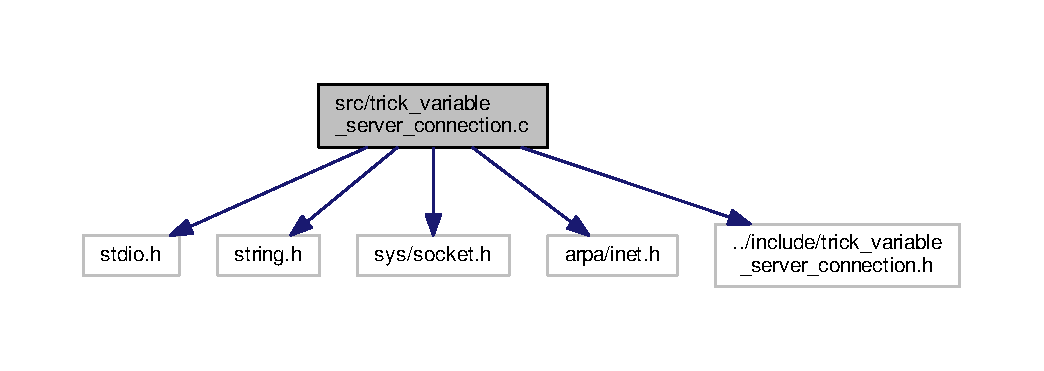
\includegraphics[width=350pt]{trick__variable__server__connection_8c__incl}
\end{center}
\end{figure}
\subsection*{Functions}
\begin{DoxyCompactItemize}
\item 
int \hyperlink{trick__variable__server__connection_8c_ad7a0b297eb139f3828ebe09af75a6faa}{create\+\_\+default\+\_\+socket} ()
\item 
int \hyperlink{trick__variable__server__connection_8c_aaf3959e7b372c6dff06f26aa8d195e4f}{create\+\_\+generic\+\_\+socket} (int domain, int type, int protocol)
\item 
int \hyperlink{trick__variable__server__connection_8c_ac39b91446fd41bcea947d7b52eb8ea42}{connect\+\_\+to\+\_\+variable\+\_\+server} (int socket, char $\ast$host, int port)
\item 
int \hyperlink{trick__variable__server__connection_8c_ae7829b090401d6dc53c4e0d2704139d2}{send\+\_\+command\+\_\+to\+\_\+variable\+\_\+server} (int socket, char $\ast$command)
\item 
int \hyperlink{trick__variable__server__connection_8c_a08c1fbb4195b169faf81ed45ca224a10}{set\+\_\+ascii} (int socket)
\item 
int \hyperlink{trick__variable__server__connection_8c_a3b2f16d2ec26e100597a6d236adb332b}{set\+\_\+binary} (int socket)
\item 
int \hyperlink{trick__variable__server__connection_8c_a3dc53d753dac42375d8f21b2035a3d88}{set\+\_\+binary\+\_\+no\+\_\+names} (int socket)
\item 
int \hyperlink{trick__variable__server__connection_8c_afec87919041227f0a57ddb1e2d1268f5}{set\+\_\+sync} (int socket)
\item 
int \hyperlink{trick__variable__server__connection_8c_a51ac8ab98e0c23282d8d7bd3389deff1}{pause} (int socket)
\item 
int \hyperlink{trick__variable__server__connection_8c_a3b3e785830d022d192b1ad9aa070c341}{unpause} (int socket)
\item 
int \hyperlink{trick__variable__server__connection_8c_acd094950076529e1478bc02b91b9c8c6}{add\+\_\+variable\+\_\+to\+\_\+server} (int socket, char $\ast$variable\+\_\+name)
\item 
int \hyperlink{trick__variable__server__connection_8c_a7e14adece3deb74304be6a7405a23524}{add\+\_\+variable\+\_\+to\+\_\+sever\+\_\+with\+\_\+units} (int socket, char $\ast$variable\+\_\+name, char $\ast$units)
\item 
int \hyperlink{trick__variable__server__connection_8c_a5effe2542194a311ace2151e32a8bebd}{remove\+\_\+variable\+\_\+from\+\_\+server} (int socket, char $\ast$variable\+\_\+name)
\item 
int \hyperlink{trick__variable__server__connection_8c_a5bdb44453c2831777e4bffb4b6565e36}{clear} (int socket)
\item 
int \hyperlink{trick__variable__server__connection_8c_a48ea8358c7c5034f76fb594b27d4224e}{set\+\_\+cycle} (int socket, double period)
\item 
int \hyperlink{trick__variable__server__connection_8c_af40c4d0337f46eb00b4c7c4851b5b31d}{set\+\_\+copy\+\_\+mode} (int socket, int mode)
\item 
int \hyperlink{trick__variable__server__connection_8c_a20bb43d25ab302853435cffc2166a5fe}{poll} (int socket)
\item 
int \hyperlink{trick__variable__server__connection_8c_ae7838c2133bc76f21e02c610cddb5871}{run} (int socket)
\item 
int \hyperlink{trick__variable__server__connection_8c_a53248fc5791d40e2613b41a986e9a75d}{freeze} (int socket)
\item 
int \hyperlink{trick__variable__server__connection_8c_a93c4c2af8c6ea39454519bbc6c0f3e56}{close} (int socket)
\item 
int \hyperlink{trick__variable__server__connection_8c_a193cf62c2d9934b26ab0cb7100685045}{set\+\_\+validate\+\_\+addresses} (int socket, int validate)
\item 
int \hyperlink{trick__variable__server__connection_8c_a3d11865232c4d53a7d564e440574edde}{set\+\_\+real\+\_\+time} (int socket, int enabled)
\item 
int \hyperlink{trick__variable__server__connection_8c_a55ab6a90239465b7313f2bfed17fafc8}{set\+\_\+debug\+\_\+level} (int socket, int level)
\item 
int \hyperlink{trick__variable__server__connection_8c_a96a6694dfe4fc2e98ac1f5cbab8b4555}{set\+\_\+client\+\_\+tag} (int socket, char $\ast$tag)
\item 
int \hyperlink{trick__variable__server__connection_8c_a2869328a708b21c74947f1095489c630}{receive\+\_\+message\+\_\+from\+\_\+variable\+\_\+server} (int socket, void $\ast$server\+\_\+reply, unsigned int lenght, int flags)
\item 
int \hyperlink{trick__variable__server__connection_8c_af39136525220219abf69d766b80793fc}{socket\+\_\+shutdown} (int socket)
\end{DoxyCompactItemize}


\subsection{Detailed Description}
The library provides a set of C functions to connect and interact to a Trick Variable Server. 

\begin{DoxyAuthor}{Author}
Alfredo Garro, University of Calabria (Italy), \href{mailto:alfredo.garro@unical.it}{\tt alfredo.\+garro@unical.\+it} 
\end{DoxyAuthor}
\begin{DoxyDate}{Date}
23 June 2016 
\end{DoxyDate}
\begin{DoxySeeAlso}{See also}
\href{https://github.com/nasa/Trick/wiki/Variable-Server}{\tt https\+://github.\+com/nasa/\+Trick/wiki/\+Variable-\/\+Server} for the documentation on the commands that can be sent to the Trick Variable Server. 
\end{DoxySeeAlso}


\subsection{Function Documentation}
\index{trick\+\_\+variable\+\_\+server\+\_\+connection.\+c@{trick\+\_\+variable\+\_\+server\+\_\+connection.\+c}!add\+\_\+variable\+\_\+to\+\_\+server@{add\+\_\+variable\+\_\+to\+\_\+server}}
\index{add\+\_\+variable\+\_\+to\+\_\+server@{add\+\_\+variable\+\_\+to\+\_\+server}!trick\+\_\+variable\+\_\+server\+\_\+connection.\+c@{trick\+\_\+variable\+\_\+server\+\_\+connection.\+c}}
\subsubsection[{\texorpdfstring{add\+\_\+variable\+\_\+to\+\_\+server(int socket, char $\ast$variable\+\_\+name)}{add_variable_to_server(int socket, char *variable_name)}}]{\setlength{\rightskip}{0pt plus 5cm}int add\+\_\+variable\+\_\+to\+\_\+server (
\begin{DoxyParamCaption}
\item[{int}]{socket, }
\item[{char $\ast$}]{variable\+\_\+name}
\end{DoxyParamCaption}
)}\hypertarget{trick__variable__server__connection_8c_acd094950076529e1478bc02b91b9c8c6}{}\label{trick__variable__server__connection_8c_acd094950076529e1478bc02b91b9c8c6}
\subsubsection*{Function\+: add\+\_\+variable\+\_\+to\+\_\+server }

adds the named variable to be observed through the Trick Variable Server.


\begin{DoxyParams}{Parameters}
{\em socket} & socket file descriptor; \\
\hline
{\em variable\+\_\+name} & name of the variable to be observed.\\
\hline
\end{DoxyParams}
\begin{DoxyReturn}{Returns}
Upon successful completion, the function returns 0. Otherwise, -\/1 is returned and errno is set to indicate the error. 
\end{DoxyReturn}
\index{trick\+\_\+variable\+\_\+server\+\_\+connection.\+c@{trick\+\_\+variable\+\_\+server\+\_\+connection.\+c}!add\+\_\+variable\+\_\+to\+\_\+sever\+\_\+with\+\_\+units@{add\+\_\+variable\+\_\+to\+\_\+sever\+\_\+with\+\_\+units}}
\index{add\+\_\+variable\+\_\+to\+\_\+sever\+\_\+with\+\_\+units@{add\+\_\+variable\+\_\+to\+\_\+sever\+\_\+with\+\_\+units}!trick\+\_\+variable\+\_\+server\+\_\+connection.\+c@{trick\+\_\+variable\+\_\+server\+\_\+connection.\+c}}
\subsubsection[{\texorpdfstring{add\+\_\+variable\+\_\+to\+\_\+sever\+\_\+with\+\_\+units(int socket, char $\ast$variable\+\_\+name, char $\ast$units)}{add_variable_to_sever_with_units(int socket, char *variable_name, char *units)}}]{\setlength{\rightskip}{0pt plus 5cm}int add\+\_\+variable\+\_\+to\+\_\+sever\+\_\+with\+\_\+units (
\begin{DoxyParamCaption}
\item[{int}]{socket, }
\item[{char $\ast$}]{variable\+\_\+name, }
\item[{char $\ast$}]{units}
\end{DoxyParamCaption}
)}\hypertarget{trick__variable__server__connection_8c_a7e14adece3deb74304be6a7405a23524}{}\label{trick__variable__server__connection_8c_a7e14adece3deb74304be6a7405a23524}
\subsubsection*{Function\+: add\+\_\+variable\+\_\+to\+\_\+server\+\_\+with\+\_\+units }

adds the named variable to be observed through the Trick Variable Server specifying the units of measure.


\begin{DoxyParams}{Parameters}
{\em socket} & socket file descriptor; \\
\hline
{\em variable\+\_\+name} & name of the variable to be observed; \\
\hline
{\em units} & units of measure of the variable to be observed.\\
\hline
\end{DoxyParams}
\begin{DoxyReturn}{Returns}
Upon successful completion, the function returns 0. Otherwise, -\/1 is returned and errno is set to indicate the error. 
\end{DoxyReturn}
\index{trick\+\_\+variable\+\_\+server\+\_\+connection.\+c@{trick\+\_\+variable\+\_\+server\+\_\+connection.\+c}!clear@{clear}}
\index{clear@{clear}!trick\+\_\+variable\+\_\+server\+\_\+connection.\+c@{trick\+\_\+variable\+\_\+server\+\_\+connection.\+c}}
\subsubsection[{\texorpdfstring{clear(int socket)}{clear(int socket)}}]{\setlength{\rightskip}{0pt plus 5cm}int clear (
\begin{DoxyParamCaption}
\item[{int}]{socket}
\end{DoxyParamCaption}
)}\hypertarget{trick__variable__server__connection_8c_a5bdb44453c2831777e4bffb4b6565e36}{}\label{trick__variable__server__connection_8c_a5bdb44453c2831777e4bffb4b6565e36}
\subsubsection*{Function\+: clear }

clears all the variables from the Trick Variable Server.


\begin{DoxyParams}{Parameters}
{\em socket} & socket file descriptor.\\
\hline
\end{DoxyParams}
\begin{DoxyReturn}{Returns}
Upon successful completion, the function returns 0. Otherwise, -\/1 is returned and errno is set to indicate the error. 
\end{DoxyReturn}
\index{trick\+\_\+variable\+\_\+server\+\_\+connection.\+c@{trick\+\_\+variable\+\_\+server\+\_\+connection.\+c}!close@{close}}
\index{close@{close}!trick\+\_\+variable\+\_\+server\+\_\+connection.\+c@{trick\+\_\+variable\+\_\+server\+\_\+connection.\+c}}
\subsubsection[{\texorpdfstring{close(int socket)}{close(int socket)}}]{\setlength{\rightskip}{0pt plus 5cm}int close (
\begin{DoxyParamCaption}
\item[{int}]{socket}
\end{DoxyParamCaption}
)}\hypertarget{trick__variable__server__connection_8c_a93c4c2af8c6ea39454519bbc6c0f3e56}{}\label{trick__variable__server__connection_8c_a93c4c2af8c6ea39454519bbc6c0f3e56}
\subsubsection*{Function\+: close }

closes the connection to the Trick Variable Server.


\begin{DoxyParams}{Parameters}
{\em socket} & socket file descriptor.\\
\hline
\end{DoxyParams}
\begin{DoxyReturn}{Returns}
Upon successful completion, the function returns 0. Otherwise, -\/1 is returned and errno is set to indicate the error. 
\end{DoxyReturn}
\index{trick\+\_\+variable\+\_\+server\+\_\+connection.\+c@{trick\+\_\+variable\+\_\+server\+\_\+connection.\+c}!connect\+\_\+to\+\_\+variable\+\_\+server@{connect\+\_\+to\+\_\+variable\+\_\+server}}
\index{connect\+\_\+to\+\_\+variable\+\_\+server@{connect\+\_\+to\+\_\+variable\+\_\+server}!trick\+\_\+variable\+\_\+server\+\_\+connection.\+c@{trick\+\_\+variable\+\_\+server\+\_\+connection.\+c}}
\subsubsection[{\texorpdfstring{connect\+\_\+to\+\_\+variable\+\_\+server(int socket, char $\ast$host, int port)}{connect_to_variable_server(int socket, char *host, int port)}}]{\setlength{\rightskip}{0pt plus 5cm}int connect\+\_\+to\+\_\+variable\+\_\+server (
\begin{DoxyParamCaption}
\item[{int}]{socket, }
\item[{char $\ast$}]{host, }
\item[{int}]{port}
\end{DoxyParamCaption}
)}\hypertarget{trick__variable__server__connection_8c_ac39b91446fd41bcea947d7b52eb8ea42}{}\label{trick__variable__server__connection_8c_ac39b91446fd41bcea947d7b52eb8ea42}
\subsubsection*{Function\+: connect\+\_\+to\+\_\+variable\+\_\+server }

Connect to the Trick Variable Server on the given host and port.


\begin{DoxyParams}{Parameters}
{\em socket} & socket file descriptor; \\
\hline
{\em host} & host I\+Pv4 address; \\
\hline
{\em port} & service port number.\\
\hline
\end{DoxyParams}
\begin{DoxyReturn}{Returns}
Upon successful completion, the function returns 0. Otherwise, -\/1 is returned and errno is set to indicate the error. 
\end{DoxyReturn}
\index{trick\+\_\+variable\+\_\+server\+\_\+connection.\+c@{trick\+\_\+variable\+\_\+server\+\_\+connection.\+c}!create\+\_\+default\+\_\+socket@{create\+\_\+default\+\_\+socket}}
\index{create\+\_\+default\+\_\+socket@{create\+\_\+default\+\_\+socket}!trick\+\_\+variable\+\_\+server\+\_\+connection.\+c@{trick\+\_\+variable\+\_\+server\+\_\+connection.\+c}}
\subsubsection[{\texorpdfstring{create\+\_\+default\+\_\+socket()}{create_default_socket()}}]{\setlength{\rightskip}{0pt plus 5cm}int create\+\_\+default\+\_\+socket (
\begin{DoxyParamCaption}
{}
\end{DoxyParamCaption}
)}\hypertarget{trick__variable__server__connection_8c_ad7a0b297eb139f3828ebe09af75a6faa}{}\label{trick__variable__server__connection_8c_ad7a0b297eb139f3828ebe09af75a6faa}
\subsubsection*{Function\+: create\+\_\+default\+\_\+socket }

Create a socket to connect to the Trick Variable Server on the given host and port with the following default parameters\+:

domain\+: {\ttfamily A\+F\+\_\+\+I\+N\+ET} (Internet address); type\+: {\ttfamily S\+O\+C\+K\+\_\+\+S\+T\+R\+E\+AM}, which provides sequenced, reliable, bidirectional, connection-\/mode byte streams, and may provide a transmission mechanism for out-\/of-\/band data; protocol\+: 0, which causes to use an unspecified default protocol appropriate for the requested socket type. \begin{DoxyReturn}{Returns}
Upon successful completion, the fuction returns a nonnegative integer, the socket file descriptor. Otherwise a value of -\/1 is returned and errno is set to indicate the error. 
\end{DoxyReturn}
\index{trick\+\_\+variable\+\_\+server\+\_\+connection.\+c@{trick\+\_\+variable\+\_\+server\+\_\+connection.\+c}!create\+\_\+generic\+\_\+socket@{create\+\_\+generic\+\_\+socket}}
\index{create\+\_\+generic\+\_\+socket@{create\+\_\+generic\+\_\+socket}!trick\+\_\+variable\+\_\+server\+\_\+connection.\+c@{trick\+\_\+variable\+\_\+server\+\_\+connection.\+c}}
\subsubsection[{\texorpdfstring{create\+\_\+generic\+\_\+socket(int domain, int type, int protocol)}{create_generic_socket(int domain, int type, int protocol)}}]{\setlength{\rightskip}{0pt plus 5cm}int create\+\_\+generic\+\_\+socket (
\begin{DoxyParamCaption}
\item[{int}]{domain, }
\item[{int}]{type, }
\item[{int}]{protocol}
\end{DoxyParamCaption}
)}\hypertarget{trick__variable__server__connection_8c_aaf3959e7b372c6dff06f26aa8d195e4f}{}\label{trick__variable__server__connection_8c_aaf3959e7b372c6dff06f26aa8d195e4f}
\subsubsection*{Function\+: create\+\_\+generic\+\_\+socket }

create a socket to connect to the Trick Variable Server on the given host and port with a set of user specified parameters.


\begin{DoxyParams}{Parameters}
{\em domain} & which can be {\ttfamily A\+F\+\_\+\+I\+N\+ET} (Internet adress) or {\ttfamily A\+F\+\_\+\+U\+N\+IX} (File system pathnames); \\
\hline
{\em type} & which can be {\ttfamily S\+O\+C\+K\+\_\+\+S\+T\+R\+E\+AM} (that Provides sequenced, reliable, bidirectional, connection-\/mode byte streams, and may provide a transmission mechanism for out-\/of-\/band data); {\ttfamily S\+O\+C\+K\+\_\+\+D\+G\+R\+AM} (that Provides datagrams, which are connectionless-\/mode, unreliable messages of fixed maximum length); {\ttfamily S\+O\+C\+K\+\_\+\+S\+E\+Q\+P\+A\+C\+K\+ET} (that Provides sequenced, reliable, bidirectional, connection-\/mode transmission path for records. A record can be sent using one or more output operations and received using one or more input operations, but a single operation never transfers part of more than one record. Record boundaries are visible to the receiver via the {\ttfamily M\+S\+G\+\_\+\+E\+OR} flag); \\
\hline
{\em protocol} & which, if non-\/zero, must specify a protocol supported by the address family.\\
\hline
\end{DoxyParams}
\begin{DoxyReturn}{Returns}
Upon successful completion, the fuction returns a nonnegative integer, the socket file descriptor. Otherwise a value of -\/1 is returned and errno is set to indicate the error. 
\end{DoxyReturn}
\index{trick\+\_\+variable\+\_\+server\+\_\+connection.\+c@{trick\+\_\+variable\+\_\+server\+\_\+connection.\+c}!freeze@{freeze}}
\index{freeze@{freeze}!trick\+\_\+variable\+\_\+server\+\_\+connection.\+c@{trick\+\_\+variable\+\_\+server\+\_\+connection.\+c}}
\subsubsection[{\texorpdfstring{freeze(int socket)}{freeze(int socket)}}]{\setlength{\rightskip}{0pt plus 5cm}int freeze (
\begin{DoxyParamCaption}
\item[{int}]{socket}
\end{DoxyParamCaption}
)}\hypertarget{trick__variable__server__connection_8c_a53248fc5791d40e2613b41a986e9a75d}{}\label{trick__variable__server__connection_8c_a53248fc5791d40e2613b41a986e9a75d}
\subsubsection*{Function\+: freeze }

sends a freeze command to the simulation.


\begin{DoxyParams}{Parameters}
{\em socket} & socket file descriptor.\\
\hline
\end{DoxyParams}
\begin{DoxyReturn}{Returns}
Upon successful completion, the function returns 0. Otherwise, -\/1 is returned and errno is set to indicate the error. 
\end{DoxyReturn}
\index{trick\+\_\+variable\+\_\+server\+\_\+connection.\+c@{trick\+\_\+variable\+\_\+server\+\_\+connection.\+c}!pause@{pause}}
\index{pause@{pause}!trick\+\_\+variable\+\_\+server\+\_\+connection.\+c@{trick\+\_\+variable\+\_\+server\+\_\+connection.\+c}}
\subsubsection[{\texorpdfstring{pause(int socket)}{pause(int socket)}}]{\setlength{\rightskip}{0pt plus 5cm}int pause (
\begin{DoxyParamCaption}
\item[{int}]{socket}
\end{DoxyParamCaption}
)}\hypertarget{trick__variable__server__connection_8c_a51ac8ab98e0c23282d8d7bd3389deff1}{}\label{trick__variable__server__connection_8c_a51ac8ab98e0c23282d8d7bd3389deff1}
\subsubsection*{Function\+: pause }

commands the Trick Variable Server to stop sending data.


\begin{DoxyParams}{Parameters}
{\em socket} & socket file descriptor.\\
\hline
\end{DoxyParams}
\begin{DoxyReturn}{Returns}
Upon successful completion, the function returns 0. Otherwise, -\/1 is returned and errno is set to indicate the error. 
\end{DoxyReturn}
\index{trick\+\_\+variable\+\_\+server\+\_\+connection.\+c@{trick\+\_\+variable\+\_\+server\+\_\+connection.\+c}!poll@{poll}}
\index{poll@{poll}!trick\+\_\+variable\+\_\+server\+\_\+connection.\+c@{trick\+\_\+variable\+\_\+server\+\_\+connection.\+c}}
\subsubsection[{\texorpdfstring{poll(int socket)}{poll(int socket)}}]{\setlength{\rightskip}{0pt plus 5cm}int poll (
\begin{DoxyParamCaption}
\item[{int}]{socket}
\end{DoxyParamCaption}
)}\hypertarget{trick__variable__server__connection_8c_a20bb43d25ab302853435cffc2166a5fe}{}\label{trick__variable__server__connection_8c_a20bb43d25ab302853435cffc2166a5fe}
\subsubsection*{Function\+: poll }

requests a single update from the Trick Variable Server.


\begin{DoxyParams}{Parameters}
{\em socket} & socket file descriptor.\\
\hline
\end{DoxyParams}
\begin{DoxyReturn}{Returns}
Upon successful completion, the function returns 0. Otherwise, -\/1 is returned and errno is set to indicate the error. 
\end{DoxyReturn}
\index{trick\+\_\+variable\+\_\+server\+\_\+connection.\+c@{trick\+\_\+variable\+\_\+server\+\_\+connection.\+c}!receive\+\_\+message\+\_\+from\+\_\+variable\+\_\+server@{receive\+\_\+message\+\_\+from\+\_\+variable\+\_\+server}}
\index{receive\+\_\+message\+\_\+from\+\_\+variable\+\_\+server@{receive\+\_\+message\+\_\+from\+\_\+variable\+\_\+server}!trick\+\_\+variable\+\_\+server\+\_\+connection.\+c@{trick\+\_\+variable\+\_\+server\+\_\+connection.\+c}}
\subsubsection[{\texorpdfstring{receive\+\_\+message\+\_\+from\+\_\+variable\+\_\+server(int socket, void $\ast$server\+\_\+reply, unsigned int lenght, int flags)}{receive_message_from_variable_server(int socket, void *server_reply, unsigned int lenght, int flags)}}]{\setlength{\rightskip}{0pt plus 5cm}int receive\+\_\+message\+\_\+from\+\_\+variable\+\_\+server (
\begin{DoxyParamCaption}
\item[{int}]{socket, }
\item[{void $\ast$}]{server\+\_\+reply, }
\item[{unsigned int}]{lenght, }
\item[{int}]{flags}
\end{DoxyParamCaption}
)}\hypertarget{trick__variable__server__connection_8c_a2869328a708b21c74947f1095489c630}{}\label{trick__variable__server__connection_8c_a2869328a708b21c74947f1095489c630}
\subsubsection*{Function\+: receive\+\_\+message\+\_\+from\+\_\+variable\+\_\+server }

receives a message from the Trick Variable Server


\begin{DoxyParams}{Parameters}
{\em socket} & socket file descriptor; \\
\hline
{\em server\+\_\+reply} & a buffer where the message from the server will be stored; \\
\hline
{\em lenght} & the length in bytes of the buffer pointed to by the server\+\_\+reply argument \\
\hline
{\em flags} & Specifies the type of message reception. Values of this argument are formed by logically OR\textquotesingle{}ing zero or more of the following values\+: {\ttfamily M\+S\+G\+\_\+\+P\+E\+EK} (peeks at an incoming message. The data is treated as unread and the next call will still return this data); {\ttfamily M\+S\+G\+\_\+\+O\+OB} (requests out-\/of-\/band data. The significance and semantics of out-\/of-\/band data are protocol-\/specific); {\ttfamily M\+S\+G\+\_\+\+W\+A\+I\+T\+A\+LL} (requests that the function block until the full amount of data requested can be returned. The function may return a smaller amount of data if a signal is caught, if the connection is terminated, if M\+S\+G\+\_\+\+P\+E\+EK was specified, or if an error is pending for the socket).\\
\hline
\end{DoxyParams}
\begin{DoxyReturn}{Returns}
Upon successful completion, the fuction returns the length of the message in bytes. If no messages are available to be received and the peer has performed an orderly shutdown, the method returns 0. Otherwise, -\/1 is returned and errno is set to indicate the error. 
\end{DoxyReturn}
\index{trick\+\_\+variable\+\_\+server\+\_\+connection.\+c@{trick\+\_\+variable\+\_\+server\+\_\+connection.\+c}!remove\+\_\+variable\+\_\+from\+\_\+server@{remove\+\_\+variable\+\_\+from\+\_\+server}}
\index{remove\+\_\+variable\+\_\+from\+\_\+server@{remove\+\_\+variable\+\_\+from\+\_\+server}!trick\+\_\+variable\+\_\+server\+\_\+connection.\+c@{trick\+\_\+variable\+\_\+server\+\_\+connection.\+c}}
\subsubsection[{\texorpdfstring{remove\+\_\+variable\+\_\+from\+\_\+server(int socket, char $\ast$variable\+\_\+name)}{remove_variable_from_server(int socket, char *variable_name)}}]{\setlength{\rightskip}{0pt plus 5cm}int remove\+\_\+variable\+\_\+from\+\_\+server (
\begin{DoxyParamCaption}
\item[{int}]{socket, }
\item[{char $\ast$}]{variable\+\_\+name}
\end{DoxyParamCaption}
)}\hypertarget{trick__variable__server__connection_8c_a5effe2542194a311ace2151e32a8bebd}{}\label{trick__variable__server__connection_8c_a5effe2542194a311ace2151e32a8bebd}
\subsubsection*{Function\+: remove\+\_\+variable\+\_\+from\+\_\+server }

removes the named variable observed through the Trick Variable Server.


\begin{DoxyParams}{Parameters}
{\em socket} & socket file descriptor; \\
\hline
{\em variable\+\_\+name} & name of the variable to stop observing.\\
\hline
\end{DoxyParams}
\begin{DoxyReturn}{Returns}
Upon successful completion, the function returns 0. Otherwise, -\/1 is returned and errno is set to indicate the error. 
\end{DoxyReturn}
\index{trick\+\_\+variable\+\_\+server\+\_\+connection.\+c@{trick\+\_\+variable\+\_\+server\+\_\+connection.\+c}!run@{run}}
\index{run@{run}!trick\+\_\+variable\+\_\+server\+\_\+connection.\+c@{trick\+\_\+variable\+\_\+server\+\_\+connection.\+c}}
\subsubsection[{\texorpdfstring{run(int socket)}{run(int socket)}}]{\setlength{\rightskip}{0pt plus 5cm}int run (
\begin{DoxyParamCaption}
\item[{int}]{socket}
\end{DoxyParamCaption}
)}\hypertarget{trick__variable__server__connection_8c_ae7838c2133bc76f21e02c610cddb5871}{}\label{trick__variable__server__connection_8c_ae7838c2133bc76f21e02c610cddb5871}
\subsubsection*{Function\+: run }

sends a run command to the simulation.


\begin{DoxyParams}{Parameters}
{\em socket} & socket file descriptor.\\
\hline
\end{DoxyParams}
\begin{DoxyReturn}{Returns}
Upon successful completion, the function returns 0. Otherwise, -\/1 is returned and errno is set to indicate the error. 
\end{DoxyReturn}
\index{trick\+\_\+variable\+\_\+server\+\_\+connection.\+c@{trick\+\_\+variable\+\_\+server\+\_\+connection.\+c}!send\+\_\+command\+\_\+to\+\_\+variable\+\_\+server@{send\+\_\+command\+\_\+to\+\_\+variable\+\_\+server}}
\index{send\+\_\+command\+\_\+to\+\_\+variable\+\_\+server@{send\+\_\+command\+\_\+to\+\_\+variable\+\_\+server}!trick\+\_\+variable\+\_\+server\+\_\+connection.\+c@{trick\+\_\+variable\+\_\+server\+\_\+connection.\+c}}
\subsubsection[{\texorpdfstring{send\+\_\+command\+\_\+to\+\_\+variable\+\_\+server(int socket, char $\ast$command)}{send_command_to_variable_server(int socket, char *command)}}]{\setlength{\rightskip}{0pt plus 5cm}int send\+\_\+command\+\_\+to\+\_\+variable\+\_\+server (
\begin{DoxyParamCaption}
\item[{int}]{socket, }
\item[{char $\ast$}]{command}
\end{DoxyParamCaption}
)}\hypertarget{trick__variable__server__connection_8c_ae7829b090401d6dc53c4e0d2704139d2}{}\label{trick__variable__server__connection_8c_ae7829b090401d6dc53c4e0d2704139d2}
\subsubsection*{Function\+: send\+\_\+command\+\_\+to\+\_\+variable\+\_\+server }

sends the given command and any commands to the Trick Variable Server A newline is automatically appended to the given command.


\begin{DoxyParams}{Parameters}
{\em socket} & socket file descriptor; \\
\hline
{\em command} & the comand to send.\\
\hline
\end{DoxyParams}
\begin{DoxyReturn}{Returns}
Upon successful completion, the function returns the number of bytes sent. Otherwise, -\/1 is returned and errno is set to indicate the error. 
\end{DoxyReturn}
\index{trick\+\_\+variable\+\_\+server\+\_\+connection.\+c@{trick\+\_\+variable\+\_\+server\+\_\+connection.\+c}!set\+\_\+ascii@{set\+\_\+ascii}}
\index{set\+\_\+ascii@{set\+\_\+ascii}!trick\+\_\+variable\+\_\+server\+\_\+connection.\+c@{trick\+\_\+variable\+\_\+server\+\_\+connection.\+c}}
\subsubsection[{\texorpdfstring{set\+\_\+ascii(int socket)}{set_ascii(int socket)}}]{\setlength{\rightskip}{0pt plus 5cm}int set\+\_\+ascii (
\begin{DoxyParamCaption}
\item[{int}]{socket}
\end{DoxyParamCaption}
)}\hypertarget{trick__variable__server__connection_8c_a08c1fbb4195b169faf81ed45ca224a10}{}\label{trick__variable__server__connection_8c_a08c1fbb4195b169faf81ed45ca224a10}
\subsubsection*{Function\+: set\+\_\+ascii }

commands the Trick Variable Server to send variable data in A\+S\+C\+II.


\begin{DoxyParams}{Parameters}
{\em socket} & socket file descriptor.\\
\hline
\end{DoxyParams}
\begin{DoxyReturn}{Returns}
Upon successful completion, the function returns 0. Otherwise, -\/1 is returned and errno is set to indicate the error. 
\end{DoxyReturn}
\index{trick\+\_\+variable\+\_\+server\+\_\+connection.\+c@{trick\+\_\+variable\+\_\+server\+\_\+connection.\+c}!set\+\_\+binary@{set\+\_\+binary}}
\index{set\+\_\+binary@{set\+\_\+binary}!trick\+\_\+variable\+\_\+server\+\_\+connection.\+c@{trick\+\_\+variable\+\_\+server\+\_\+connection.\+c}}
\subsubsection[{\texorpdfstring{set\+\_\+binary(int socket)}{set_binary(int socket)}}]{\setlength{\rightskip}{0pt plus 5cm}int set\+\_\+binary (
\begin{DoxyParamCaption}
\item[{int}]{socket}
\end{DoxyParamCaption}
)}\hypertarget{trick__variable__server__connection_8c_a3b2f16d2ec26e100597a6d236adb332b}{}\label{trick__variable__server__connection_8c_a3b2f16d2ec26e100597a6d236adb332b}
\subsubsection*{Function\+: set\+\_\+binary }

commands the Trick Variable Server to send variable data in B\+I\+N\+A\+RY.


\begin{DoxyParams}{Parameters}
{\em socket} & socket file descriptor.\\
\hline
\end{DoxyParams}
\begin{DoxyReturn}{Returns}
Upon successful completion, the function returns 0. Otherwise, -\/1 is returned and errno is set to indicate the error. 
\end{DoxyReturn}
\index{trick\+\_\+variable\+\_\+server\+\_\+connection.\+c@{trick\+\_\+variable\+\_\+server\+\_\+connection.\+c}!set\+\_\+binary\+\_\+no\+\_\+names@{set\+\_\+binary\+\_\+no\+\_\+names}}
\index{set\+\_\+binary\+\_\+no\+\_\+names@{set\+\_\+binary\+\_\+no\+\_\+names}!trick\+\_\+variable\+\_\+server\+\_\+connection.\+c@{trick\+\_\+variable\+\_\+server\+\_\+connection.\+c}}
\subsubsection[{\texorpdfstring{set\+\_\+binary\+\_\+no\+\_\+names(int socket)}{set_binary_no_names(int socket)}}]{\setlength{\rightskip}{0pt plus 5cm}int set\+\_\+binary\+\_\+no\+\_\+names (
\begin{DoxyParamCaption}
\item[{int}]{socket}
\end{DoxyParamCaption}
)}\hypertarget{trick__variable__server__connection_8c_a3dc53d753dac42375d8f21b2035a3d88}{}\label{trick__variable__server__connection_8c_a3dc53d753dac42375d8f21b2035a3d88}
\subsubsection*{Function\+: set\+\_\+binary\+\_\+no\+\_\+names }

commands the Trick Variable Server to send variable data in binary and to omit names.


\begin{DoxyParams}{Parameters}
{\em socket} & socket file descriptor.\\
\hline
\end{DoxyParams}
\begin{DoxyReturn}{Returns}
Upon successful completion, the function returns 0. Otherwise, -\/1 is returned and errno is set to indicate the error. 
\end{DoxyReturn}
\index{trick\+\_\+variable\+\_\+server\+\_\+connection.\+c@{trick\+\_\+variable\+\_\+server\+\_\+connection.\+c}!set\+\_\+client\+\_\+tag@{set\+\_\+client\+\_\+tag}}
\index{set\+\_\+client\+\_\+tag@{set\+\_\+client\+\_\+tag}!trick\+\_\+variable\+\_\+server\+\_\+connection.\+c@{trick\+\_\+variable\+\_\+server\+\_\+connection.\+c}}
\subsubsection[{\texorpdfstring{set\+\_\+client\+\_\+tag(int socket, char $\ast$tag)}{set_client_tag(int socket, char *tag)}}]{\setlength{\rightskip}{0pt plus 5cm}int set\+\_\+client\+\_\+tag (
\begin{DoxyParamCaption}
\item[{int}]{socket, }
\item[{char $\ast$}]{tag}
\end{DoxyParamCaption}
)}\hypertarget{trick__variable__server__connection_8c_a96a6694dfe4fc2e98ac1f5cbab8b4555}{}\label{trick__variable__server__connection_8c_a96a6694dfe4fc2e98ac1f5cbab8b4555}
\subsubsection*{Function\+: set\+\_\+client\+\_\+tag }

sets this client\textquotesingle{}s tag


\begin{DoxyParams}{Parameters}
{\em socket} & socket file descriptor; \\
\hline
{\em tag} & the client\textquotesingle{}s tag to set.\\
\hline
\end{DoxyParams}
\begin{DoxyReturn}{Returns}
Upon successful completion, the function returns 0. Otherwise, -\/1 is returned and errno is set to indicate the error. 
\end{DoxyReturn}
\index{trick\+\_\+variable\+\_\+server\+\_\+connection.\+c@{trick\+\_\+variable\+\_\+server\+\_\+connection.\+c}!set\+\_\+copy\+\_\+mode@{set\+\_\+copy\+\_\+mode}}
\index{set\+\_\+copy\+\_\+mode@{set\+\_\+copy\+\_\+mode}!trick\+\_\+variable\+\_\+server\+\_\+connection.\+c@{trick\+\_\+variable\+\_\+server\+\_\+connection.\+c}}
\subsubsection[{\texorpdfstring{set\+\_\+copy\+\_\+mode(int socket, int mode)}{set_copy_mode(int socket, int mode)}}]{\setlength{\rightskip}{0pt plus 5cm}int set\+\_\+copy\+\_\+mode (
\begin{DoxyParamCaption}
\item[{int}]{socket, }
\item[{int}]{mode}
\end{DoxyParamCaption}
)}\hypertarget{trick__variable__server__connection_8c_af40c4d0337f46eb00b4c7c4851b5b31d}{}\label{trick__variable__server__connection_8c_af40c4d0337f46eb00b4c7c4851b5b31d}
\subsubsection*{Function\+: set\+\_\+copy\+\_\+mode }

sets how values are copied out of the simulation by the Trick Variable Server.


\begin{DoxyParams}{Parameters}
{\em socket} & socket file descriptor; \\
\hline
{\em mode} & 0 (values are copied out of the sim asynchronously); 1 (values are copied at the end of execution frame); 2 (copies are done at a multiple and offset of the Executive software frame).\\
\hline
\end{DoxyParams}
\begin{DoxyReturn}{Returns}
Upon successful completion, the function returns 0. Otherwise, -\/1 is returned and errno is set to indicate the error. 
\end{DoxyReturn}
\index{trick\+\_\+variable\+\_\+server\+\_\+connection.\+c@{trick\+\_\+variable\+\_\+server\+\_\+connection.\+c}!set\+\_\+cycle@{set\+\_\+cycle}}
\index{set\+\_\+cycle@{set\+\_\+cycle}!trick\+\_\+variable\+\_\+server\+\_\+connection.\+c@{trick\+\_\+variable\+\_\+server\+\_\+connection.\+c}}
\subsubsection[{\texorpdfstring{set\+\_\+cycle(int socket, double period)}{set_cycle(int socket, double period)}}]{\setlength{\rightskip}{0pt plus 5cm}int set\+\_\+cycle (
\begin{DoxyParamCaption}
\item[{int}]{socket, }
\item[{double}]{period}
\end{DoxyParamCaption}
)}\hypertarget{trick__variable__server__connection_8c_a48ea8358c7c5034f76fb594b27d4224e}{}\label{trick__variable__server__connection_8c_a48ea8358c7c5034f76fb594b27d4224e}
\subsubsection*{Function\+: set\+\_\+cycle }

sets the period at which the Trick Variable Server sends updates.


\begin{DoxyParams}{Parameters}
{\em socket} & socket file descriptor; \\
\hline
{\em period} & the period at which the Trick Variable Server sends updates.\\
\hline
\end{DoxyParams}
\begin{DoxyReturn}{Returns}
Upon successful completion, the function returns 0. Otherwise, -\/1 is returned and errno is set to indicate the error. 
\end{DoxyReturn}
\index{trick\+\_\+variable\+\_\+server\+\_\+connection.\+c@{trick\+\_\+variable\+\_\+server\+\_\+connection.\+c}!set\+\_\+debug\+\_\+level@{set\+\_\+debug\+\_\+level}}
\index{set\+\_\+debug\+\_\+level@{set\+\_\+debug\+\_\+level}!trick\+\_\+variable\+\_\+server\+\_\+connection.\+c@{trick\+\_\+variable\+\_\+server\+\_\+connection.\+c}}
\subsubsection[{\texorpdfstring{set\+\_\+debug\+\_\+level(int socket, int level)}{set_debug_level(int socket, int level)}}]{\setlength{\rightskip}{0pt plus 5cm}int set\+\_\+debug\+\_\+level (
\begin{DoxyParamCaption}
\item[{int}]{socket, }
\item[{int}]{level}
\end{DoxyParamCaption}
)}\hypertarget{trick__variable__server__connection_8c_a55ab6a90239465b7313f2bfed17fafc8}{}\label{trick__variable__server__connection_8c_a55ab6a90239465b7313f2bfed17fafc8}
\subsubsection*{Function\+: set\+\_\+debug\+\_\+level }

sets the Trick Variable Server\textquotesingle{}s debug level


\begin{DoxyParams}{Parameters}
{\em socket} & socket file descriptor; \\
\hline
{\em level} & the debug level.\\
\hline
\end{DoxyParams}
\begin{DoxyReturn}{Returns}
Upon successful completion, the function returns 0. Otherwise, -\/1 is returned and errno is set to indicate the error. 
\end{DoxyReturn}
\index{trick\+\_\+variable\+\_\+server\+\_\+connection.\+c@{trick\+\_\+variable\+\_\+server\+\_\+connection.\+c}!set\+\_\+real\+\_\+time@{set\+\_\+real\+\_\+time}}
\index{set\+\_\+real\+\_\+time@{set\+\_\+real\+\_\+time}!trick\+\_\+variable\+\_\+server\+\_\+connection.\+c@{trick\+\_\+variable\+\_\+server\+\_\+connection.\+c}}
\subsubsection[{\texorpdfstring{set\+\_\+real\+\_\+time(int socket, int enabled)}{set_real_time(int socket, int enabled)}}]{\setlength{\rightskip}{0pt plus 5cm}int set\+\_\+real\+\_\+time (
\begin{DoxyParamCaption}
\item[{int}]{socket, }
\item[{int}]{enabled}
\end{DoxyParamCaption}
)}\hypertarget{trick__variable__server__connection_8c_a3d11865232c4d53a7d564e440574edde}{}\label{trick__variable__server__connection_8c_a3d11865232c4d53a7d564e440574edde}
\subsubsection*{Function\+: set\+\_\+real\+\_\+time }

sends an enable or disable real time command to the simulation


\begin{DoxyParams}{Parameters}
{\em socket} & socket file descriptor; \\
\hline
{\em enabled} & 0 for validate False, $>$0 for validate True.\\
\hline
\end{DoxyParams}
\begin{DoxyReturn}{Returns}
Upon successful completion, the function returns 0. Otherwise, -\/1 is returned and errno is set to indicate the error. 
\end{DoxyReturn}
\index{trick\+\_\+variable\+\_\+server\+\_\+connection.\+c@{trick\+\_\+variable\+\_\+server\+\_\+connection.\+c}!set\+\_\+sync@{set\+\_\+sync}}
\index{set\+\_\+sync@{set\+\_\+sync}!trick\+\_\+variable\+\_\+server\+\_\+connection.\+c@{trick\+\_\+variable\+\_\+server\+\_\+connection.\+c}}
\subsubsection[{\texorpdfstring{set\+\_\+sync(int socket)}{set_sync(int socket)}}]{\setlength{\rightskip}{0pt plus 5cm}int set\+\_\+sync (
\begin{DoxyParamCaption}
\item[{int}]{socket}
\end{DoxyParamCaption}
)}\hypertarget{trick__variable__server__connection_8c_afec87919041227f0a57ddb1e2d1268f5}{}\label{trick__variable__server__connection_8c_afec87919041227f0a57ddb1e2d1268f5}
\subsubsection*{Function\+: set\+\_\+sync }

sets the Trick Variable Server to synchronized mode.


\begin{DoxyParams}{Parameters}
{\em socket} & socket file descriptor.\\
\hline
\end{DoxyParams}
\begin{DoxyReturn}{Returns}
Upon successful completion, the function returns 0. Otherwise, -\/1 is returned and errno is set to indicate the error. 
\end{DoxyReturn}
\index{trick\+\_\+variable\+\_\+server\+\_\+connection.\+c@{trick\+\_\+variable\+\_\+server\+\_\+connection.\+c}!set\+\_\+validate\+\_\+addresses@{set\+\_\+validate\+\_\+addresses}}
\index{set\+\_\+validate\+\_\+addresses@{set\+\_\+validate\+\_\+addresses}!trick\+\_\+variable\+\_\+server\+\_\+connection.\+c@{trick\+\_\+variable\+\_\+server\+\_\+connection.\+c}}
\subsubsection[{\texorpdfstring{set\+\_\+validate\+\_\+addresses(int socket, int validate)}{set_validate_addresses(int socket, int validate)}}]{\setlength{\rightskip}{0pt plus 5cm}int set\+\_\+validate\+\_\+addresses (
\begin{DoxyParamCaption}
\item[{int}]{socket, }
\item[{int}]{validate}
\end{DoxyParamCaption}
)}\hypertarget{trick__variable__server__connection_8c_a193cf62c2d9934b26ab0cb7100685045}{}\label{trick__variable__server__connection_8c_a193cf62c2d9934b26ab0cb7100685045}
\subsubsection*{Function\+: set\+\_\+validate\+\_\+addresses }

validates the addresses of the Trick Variable Server.


\begin{DoxyParams}{Parameters}
{\em socket} & socket file descriptor. \\
\hline
{\em validate} & 0 for validate False, $>$0 for validate True;\\
\hline
\end{DoxyParams}
\begin{DoxyReturn}{Returns}
Upon successful completion, the function returns 0. Otherwise, -\/1 is returned and errno is set to indicate the error. 
\end{DoxyReturn}
\index{trick\+\_\+variable\+\_\+server\+\_\+connection.\+c@{trick\+\_\+variable\+\_\+server\+\_\+connection.\+c}!socket\+\_\+shutdown@{socket\+\_\+shutdown}}
\index{socket\+\_\+shutdown@{socket\+\_\+shutdown}!trick\+\_\+variable\+\_\+server\+\_\+connection.\+c@{trick\+\_\+variable\+\_\+server\+\_\+connection.\+c}}
\subsubsection[{\texorpdfstring{socket\+\_\+shutdown(int socket)}{socket_shutdown(int socket)}}]{\setlength{\rightskip}{0pt plus 5cm}int socket\+\_\+shutdown (
\begin{DoxyParamCaption}
\item[{int}]{socket}
\end{DoxyParamCaption}
)}\hypertarget{trick__variable__server__connection_8c_af39136525220219abf69d766b80793fc}{}\label{trick__variable__server__connection_8c_af39136525220219abf69d766b80793fc}
\subsubsection*{Function\+: socket\+\_\+shutdown }

disables subsequent send and receive operations on a socket.


\begin{DoxyParams}{Parameters}
{\em socket} & socket file descriptor.\\
\hline
\end{DoxyParams}
\begin{DoxyReturn}{Returns}
Upon successful completion, the function returns 0. Otherwise, -\/1 is returned and errno is set to indicate the error. 
\end{DoxyReturn}
\index{trick\+\_\+variable\+\_\+server\+\_\+connection.\+c@{trick\+\_\+variable\+\_\+server\+\_\+connection.\+c}!unpause@{unpause}}
\index{unpause@{unpause}!trick\+\_\+variable\+\_\+server\+\_\+connection.\+c@{trick\+\_\+variable\+\_\+server\+\_\+connection.\+c}}
\subsubsection[{\texorpdfstring{unpause(int socket)}{unpause(int socket)}}]{\setlength{\rightskip}{0pt plus 5cm}int unpause (
\begin{DoxyParamCaption}
\item[{int}]{socket}
\end{DoxyParamCaption}
)}\hypertarget{trick__variable__server__connection_8c_a3b3e785830d022d192b1ad9aa070c341}{}\label{trick__variable__server__connection_8c_a3b3e785830d022d192b1ad9aa070c341}
\subsubsection*{Function\+: unpause }

commands the Trick Variable Server to resume sending data.


\begin{DoxyParams}{Parameters}
{\em socket} & socket file descriptor.\\
\hline
\end{DoxyParams}
\begin{DoxyReturn}{Returns}
Upon successful completion, the function returns 0. Otherwise, -\/1 is returned and errno is set to indicate the error. 
\end{DoxyReturn}

\hypertarget{test01__set__one__reading_8c}{}\section{test/test01\+\_\+set\+\_\+one\+\_\+reading.c File Reference}
\label{test01__set__one__reading_8c}\index{test/test01\+\_\+set\+\_\+one\+\_\+reading.\+c@{test/test01\+\_\+set\+\_\+one\+\_\+reading.\+c}}


This is a simple test that shows how to connect and interact to a Trick Variable Server for querying and reading simulation data (just one reading). The source simulation is the S\+I\+M\+\_\+cannon\+\_\+jet reported in the Trick Tutorial \char`\"{}\+Trick Simulation Environment User Training Materials Trick 2013.\+0 Release\char`\"{}, see Section 9.\+0 and subsequent. The program takes as first input parameter the port number on which the Trick Variable Server is active. The server is supposed to run locally. If not, the IP address must be provided after the port number as the second input parameter.  


{\ttfamily \#include $<$stdio.\+h$>$}\\*
{\ttfamily \#include $<$stdlib.\+h$>$}\\*
{\ttfamily \#include $<$string.\+h$>$}\\*
{\ttfamily \#include \char`\"{}../include/trick\+\_\+variable\+\_\+server\+\_\+connection.\+h\char`\"{}}\\*
Include dependency graph for test01\+\_\+set\+\_\+one\+\_\+reading.\+c\+:
\nopagebreak
\begin{figure}[H]
\begin{center}
\leavevmode
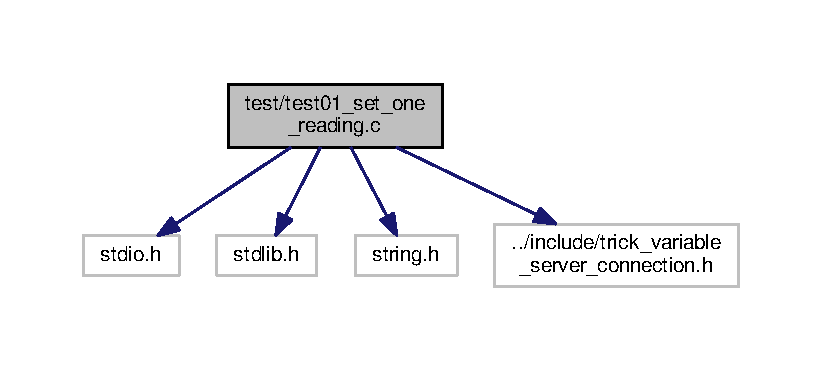
\includegraphics[width=350pt]{test01__set__one__reading_8c__incl}
\end{center}
\end{figure}
\subsection*{Functions}
\begin{DoxyCompactItemize}
\item 
int {\bfseries main} (int narg, char $\ast$$\ast$args)\hypertarget{test01__set__one__reading_8c_a8bc81d4e8cd0819680a03b135b7d6c4b}{}\label{test01__set__one__reading_8c_a8bc81d4e8cd0819680a03b135b7d6c4b}

\end{DoxyCompactItemize}


\subsection{Detailed Description}
This is a simple test that shows how to connect and interact to a Trick Variable Server for querying and reading simulation data (just one reading). The source simulation is the S\+I\+M\+\_\+cannon\+\_\+jet reported in the Trick Tutorial \char`\"{}\+Trick Simulation Environment User Training Materials Trick 2013.\+0 Release\char`\"{}, see Section 9.\+0 and subsequent. The program takes as first input parameter the port number on which the Trick Variable Server is active. The server is supposed to run locally. If not, the IP address must be provided after the port number as the second input parameter. 

\begin{DoxyAuthor}{Author}
Alfredo Garro, University of Calabria (Italy), \href{mailto:alfredo.garro@unical.it}{\tt alfredo.\+garro@unical.\+it} 
\end{DoxyAuthor}
\begin{DoxyDate}{Date}
29 June 2016 
\end{DoxyDate}
\begin{DoxySeeAlso}{See also}
\href{https://github.com/nasa/Trick/wiki/Variable-Server}{\tt https\+://github.\+com/nasa/\+Trick/wiki/\+Variable-\/\+Server} for the documentation on the commands that can be sent to the Trick Variable Server. 
\end{DoxySeeAlso}

\hypertarget{test02__set__multiple__readings_8c}{}\section{test/test02\+\_\+set\+\_\+multiple\+\_\+readings.c File Reference}
\label{test02__set__multiple__readings_8c}\index{test/test02\+\_\+set\+\_\+multiple\+\_\+readings.\+c@{test/test02\+\_\+set\+\_\+multiple\+\_\+readings.\+c}}


This is a simple test that shows how to connect and interact to a Trick Variable Server for querying and reading simulation data until they are provided by the Server. The source simulation is the S\+I\+M\+\_\+cannon\+\_\+jet reported in the Trick Tutorial \char`\"{}\+Trick Simulation Environment User Training Materials Trick 2013.\+0 Release\char`\"{}, see Section 9.\+0 and subsequent. The program takes as first input parameter the port number on which the Trick Variable Server is active. The server is supposed to run locally. If not, the IP address must be provided after the port number as the second input parameter.  


{\ttfamily \#include $<$stdio.\+h$>$}\\*
{\ttfamily \#include $<$stdlib.\+h$>$}\\*
{\ttfamily \#include $<$string.\+h$>$}\\*
{\ttfamily \#include \char`\"{}../include/trick\+\_\+variable\+\_\+server\+\_\+connection.\+h\char`\"{}}\\*
Include dependency graph for test02\+\_\+set\+\_\+multiple\+\_\+readings.\+c\+:
\nopagebreak
\begin{figure}[H]
\begin{center}
\leavevmode
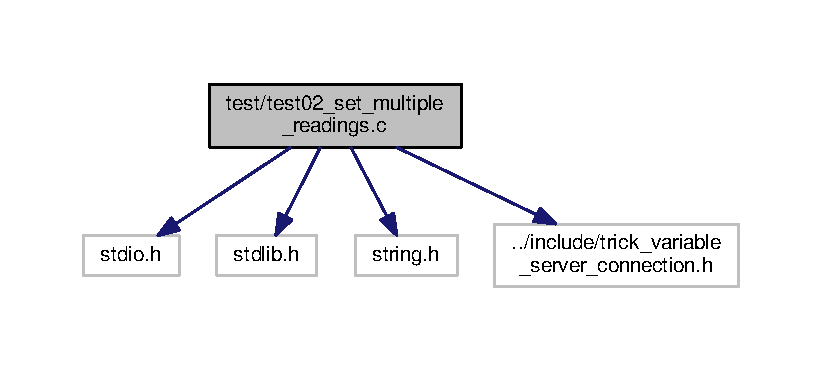
\includegraphics[width=350pt]{test02__set__multiple__readings_8c__incl}
\end{center}
\end{figure}
\subsection*{Functions}
\begin{DoxyCompactItemize}
\item 
int {\bfseries main} (int narg, char $\ast$$\ast$args)\hypertarget{test02__set__multiple__readings_8c_a8bc81d4e8cd0819680a03b135b7d6c4b}{}\label{test02__set__multiple__readings_8c_a8bc81d4e8cd0819680a03b135b7d6c4b}

\end{DoxyCompactItemize}


\subsection{Detailed Description}
This is a simple test that shows how to connect and interact to a Trick Variable Server for querying and reading simulation data until they are provided by the Server. The source simulation is the S\+I\+M\+\_\+cannon\+\_\+jet reported in the Trick Tutorial \char`\"{}\+Trick Simulation Environment User Training Materials Trick 2013.\+0 Release\char`\"{}, see Section 9.\+0 and subsequent. The program takes as first input parameter the port number on which the Trick Variable Server is active. The server is supposed to run locally. If not, the IP address must be provided after the port number as the second input parameter. 

\begin{DoxyAuthor}{Author}
Alfredo Garro, University of Calabria (Italy), \href{mailto:alfredo.garro@unical.it}{\tt alfredo.\+garro@unical.\+it} 
\end{DoxyAuthor}
\begin{DoxyDate}{Date}
29 June 2016 
\end{DoxyDate}
\begin{DoxySeeAlso}{See also}
\href{https://github.com/nasa/Trick/wiki/Variable-Server}{\tt https\+://github.\+com/nasa/\+Trick/wiki/\+Variable-\/\+Server} for the documentation on the commands that can be sent to the Trick Variable Server. 
\end{DoxySeeAlso}

%--- End generated contents ---

% Index
\backmatter
\newpage
\phantomsection
\clearemptydoublepage
\addcontentsline{toc}{chapter}{Index}
\printindex

\end{document}
